\chapter{Regressione} %\label{4cap:regressione}

\begin{preamble}
{\em In questo capitolo viene affrontato il problema della regressione poiché il dataset in esame si presta naturalmente a questo tipo di
formulazione del problema.}
\end{preamble}

La regressione è una tecnica di apprendimento supervisionato che consente
di modellare la relazione tra una variabile obiettivo continua e un
insieme di variabili input, con l'obiettivo di stimare il valore atteso
della prima condizionato ai valori assunti dalle seconde.

I task che si vogliono affrontare in questo capitolo sono i seguenti:

\begin{itemize}
    \item \textbf{T2 -- Prevedere il prezzo orario a partire dal mix di generazione}\\
    stabilire il prezzo all'ora $t$
    dalle fonti di generazione della stessa ora e dal contesto temporale.
\end{itemize}

\section{Metriche di Valutazione Scelte}
\label{sec:t2_regressione_metriche}
Per valutare i modelli sul test set (2025), sono state impiegate cinque metriche:

\begin{itemize}
    \item \textbf{Mean Absolute Error (MAE)}:
    \begin{equation}
    \text{MAE} = \frac{1}{N} \sum_{i=1}^{N} |y_i - \hat{y}_i|
    \end{equation}
    Calcolato con \texttt{mean\_absolute\_error}, esprime l'errore medio in \euro/MWh ed è robusto agli outlier.

    \item \textbf{Root Mean Squared Error (RMSE)}:
    \begin{equation}
    \text{RMSE} = \sqrt{\frac{1}{N} \sum_{i=1}^{N} (y_i - \hat{y}_i)^2}
    \end{equation}
    Calcolato con \texttt{np.sqrt(mean\_squared\_error)}, penalizza maggiormente gli scostamenti ampi e i picchi estremi.

    \item \textbf{Coefficiente di Determinazione ($R^2$)}:
    \begin{equation}
    R^2 = 1 - \frac{\sum_{i=1}^N (y_i - \hat{y}_i)^2}{\sum_{i=1}^N (y_i - \bar{y})^2}
    \end{equation}
    Calcolato con \texttt{r2\_score}, indica la quota di varianza spiegata rispetto alla media ($1$ perfetto, $\leq 0$ non informativo).

    \item \textbf{Mean Bias Error (Bias)}:
    \begin{equation}
    \text{Bias} = \frac{1}{N} \sum_{i=1}^{N} (\hat{y}_i - y_i)
    \end{equation}
    Calcolato con \texttt{np.mean(y\_pred - y\_test)}, quantifica la tendenza sistematica a sottostimare ($<0$) o sovrastimare ($>0$).

    \item \textbf{Correlazione di Spearman ($\rho$)}:
    \begin{equation}
    \rho = 1 - \frac{6 \sum_{i=1}^{N} d_i^2}{N(N^2 - 1)}
    \end{equation}
    Calcolato con \texttt{spearmanr}, misura la capacità del modello di ordinare correttamente le ore dalle più economiche alle più costose. Il termine $d_i$ rappresenta la differenza tra i ranghi delle due variabili per l'$i$-esima osservazione.
\end{itemize}

\section{Task 2: Previsione del prezzo orario a partire dal mix di generazione}
\label{sec:t2_regressione_obiettivo}

\subsection{Definizione dell'Obiettivo}
Il task predittivo \textbf{Task 2 (T2)} consiste nella stima puntuale continua del prezzo dell'energia elettrica all'ingrosso sul mercato \textit{day-ahead} per ciascuna zona di mercato $z$ all'ora $t$, basandosi unicamente sul mix di produzione elettrica per fonte e sul contesto temporale della stessa ora.

L'obiettivo di questo task è verificare se e con quale accuratezza sia possibile apprendere la funzione di costo marginale del sistema elettrico europeo in modo puramente statico (ossia senza informazioni autoregressive o lag di prezzo passati), stimando direttamente il prezzo a partire dalla composizione istantanea dell'offerta e dal ciclo di consumo intra-giornaliero e settimanale. Tale formulazione è di fondamentale rilevanza per la simulazione di scenari energetici futuri.

Matematicamente, il problema è formalizzato come una regressione supervisionata in cui la variabile target continua è:
\begin{equation}
y = P_{z,t} \in \mathbb{R} \quad [\text{\euro / MWh}]
\end{equation}
a partire da un vettore di feature $\mathbf{x} \in \mathbb{R}^{D}$ composto da:
\begin{itemize}
    \item \textbf{Mix di generazione} $\mathbf{g}_t \in \mathbb{R}^{10}$: quote orarie di produzione in MW suddivise per tecnologia (fotovoltaico, eolico onshore/offshore, nucleare, gas fossile, carbone, lignite, idroelettrico totale, biomassa e rifiuti);
    \item \textbf{Contesto temporale} $\mathbf{t}_t \in \mathbb{R}^{5}$: ora locale del giorno $h \in [0, 23]$, trasformazione ciclica $[\sin(2\pi h / 24), \cos(2\pi h / 24)]$, giorno della settimana e variabile binaria di weekend;
    \item \textbf{Localizzazione geografica} $\mathbf{z} \in \{0, 1\}^{K-1}$: codifica one-hot delle $K=22$ zone di mercato europee considerate.
\end{itemize}

L'algoritmo di regressione mira quindi ad apprendere un'ipotesi predittiva $\hat{f}: \mathcal{X} \to \mathbb{R}$ che minimizzi l'errore atteso di predizione:
\begin{equation}
\hat{y} = \hat{f}(\mathbf{x}) \approx y
\end{equation}
consentendo di quantificare la quota di varianza del prezzo spiegabile unicamente dalle caratteristiche di generazione e dal ciclo orario della domanda.

\subsection{Protocollo sperimentale}
Il dataset è stato suddiviso cronologicamente: addestramento sulle osservazioni del 2024 e test sul periodo gennaio--giugno 2025. Il test comprende 95.040 osservazioni orarie relative alle 22 zone di mercato. Le feature includono produzione per fonte, variabili temporali locali e codifica one-hot della zona; il prezzo è la variabile obiettivo. La variabile di qualità è mantenuta tra le feature, come nel notebook sperimentale.

Per ciascun modello sono riportate le metriche calcolate sull'intero test: MAE, MSE, RMSE, $R^2$, bias medio e correlazione di Spearman. Il grafico mostra un campione riproducibile di 15.000 osservazioni per facilitarne la lettura; la diagonale tratteggiata rappresenta la previsione ideale.

\newpage

\section{Random Forest}
La Random Forest è un modello di \textit{ensemble} che combina le previsioni di più alberi decisionali indipendenti, addestrati su sottoinsiemi casuali delle osservazioni e delle feature. Questa strategia riduce la varianza tipica di un singolo albero e migliora la capacità di generalizzazione. Nel nostro caso la Random Forest è stata configurata con 100 alberi decisionali e almeno cinque osservazioni per foglia; durante l'addestramento ogni albero apprende regole basate sulle feature energetiche e temporali, e la previsione sul test è ottenuta aggregando (mediando) le uscite della foresta. L'implementazione è riportata nel Codice~\ref{lst:reg_rf}.

\begin{lstlisting}[language=Python, caption={Addestramento e previsione con Random Forest.}, label={lst:reg_rf}]
rf = RandomForestRegressor(
    n_estimators=100, min_samples_leaf=5,
    n_jobs=-1, random_state=42
)
rf.fit(X_train, y_train)
y_pred = rf.predict(X_test)
\end{lstlisting}

\subsection{Metriche sul test}
La Tabella~\ref{tab:reg_metriche_rf} riporta le prestazioni sul periodo di test. Il bias negativo indica una sottostima media dei prezzi.
\begin{table}[htbp]
    \centering\small
    \begin{tabular}{|l|r|r|r|r|r|r|}\hline
    \rowcolor[gray]{0.9} Modello & MAE & MSE & RMSE & $R^2$ & Bias & Spearman \\
    \hline
    Random Forest & 29,99 & 1.726,40 & 41,55 & 0,537 & $-7,16$ & 0,775 \\
    \hline\end{tabular}
    \caption{Metriche della Random Forest sul test. MAE, RMSE e bias in \euro/MWh; MSE in $(\euro/\mathrm{MWh})^2$.}
    \label{tab:reg_metriche_rf}
\end{table}

\subsection{Grafico delle previsioni}
\begin{figure}[ht!]
    \centering
    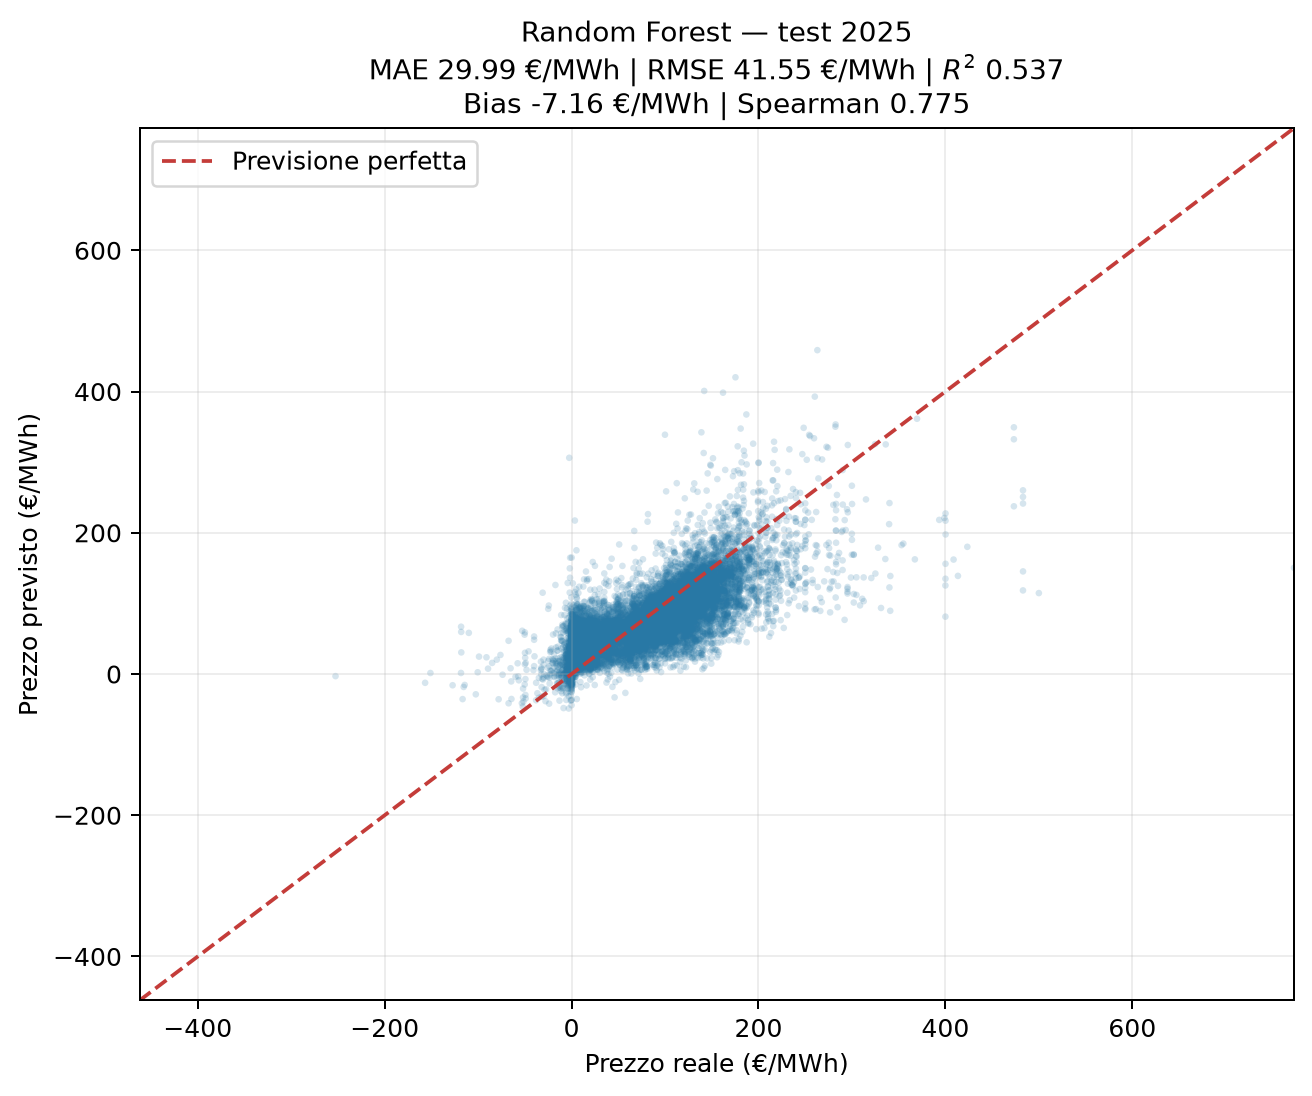
\includegraphics[width=0.78\textwidth]{images/analisi/regressione/random_forest.png}
    \caption{Prezzi reali e previsti dalla Random Forest sul test gennaio--giugno 2025.}
    \label{fig:reg_rf_test}
\end{figure}

\newpage

\section{Decision Tree}
Il Decision Tree è un modello che costruisce una sequenza gerarchica di regole if-then, suddividendo ricorsivamente lo spazio delle feature fino a formare gruppi di osservazioni omogenee. È un modello semplice e interpretabile, ma tende a overfittare se non viene potato. L'albero è stato addestrato senza un limite esplicito alla profondità, imponendo almeno cinque osservazioni per foglia. Sul training ha ottenuto MAE 10,42~\euro/MWh e $R^2=0,875$; il divario con i risultati sul test segnala overfitting e minore capacità di generalizzare al periodo successivo. Il codice di addestramento e previsione è mostrato nel Codice~\ref{lst:reg_dt}.

\begin{lstlisting}[language=Python, caption={Addestramento e previsione con Decision Tree.}, label={lst:reg_dt}]
dt = DecisionTreeRegressor(
    max_depth=None, min_samples_leaf=5,
    random_state=42
)
dt.fit(X_train, y_train)
y_pred_dt = dt.predict(X_test)
\end{lstlisting}

\subsection{Metriche sul test}
\begin{table}[htbp]
    \centering\small
    \begin{tabular}{|l|r|r|r|r|r|r|}\hline
    \rowcolor[gray]{0.9} Modello & MAE & MSE & RMSE & $R^2$ & Bias & Spearman \\
    \hline
    Decision Tree & 36,55 & 2.895,97 & 53,81 & 0,224 & $-7,49$ & 0,674 \\
    \hline\end{tabular}
    \caption{Metriche del Decision Tree sul test. MAE, RMSE e bias in \euro/MWh; MSE in $(\euro/\mathrm{MWh})^2$.}
    \label{tab:reg_metriche_dt}
\end{table}

\subsection{Grafico delle previsioni}
\begin{figure}[ht!]
    \centering
    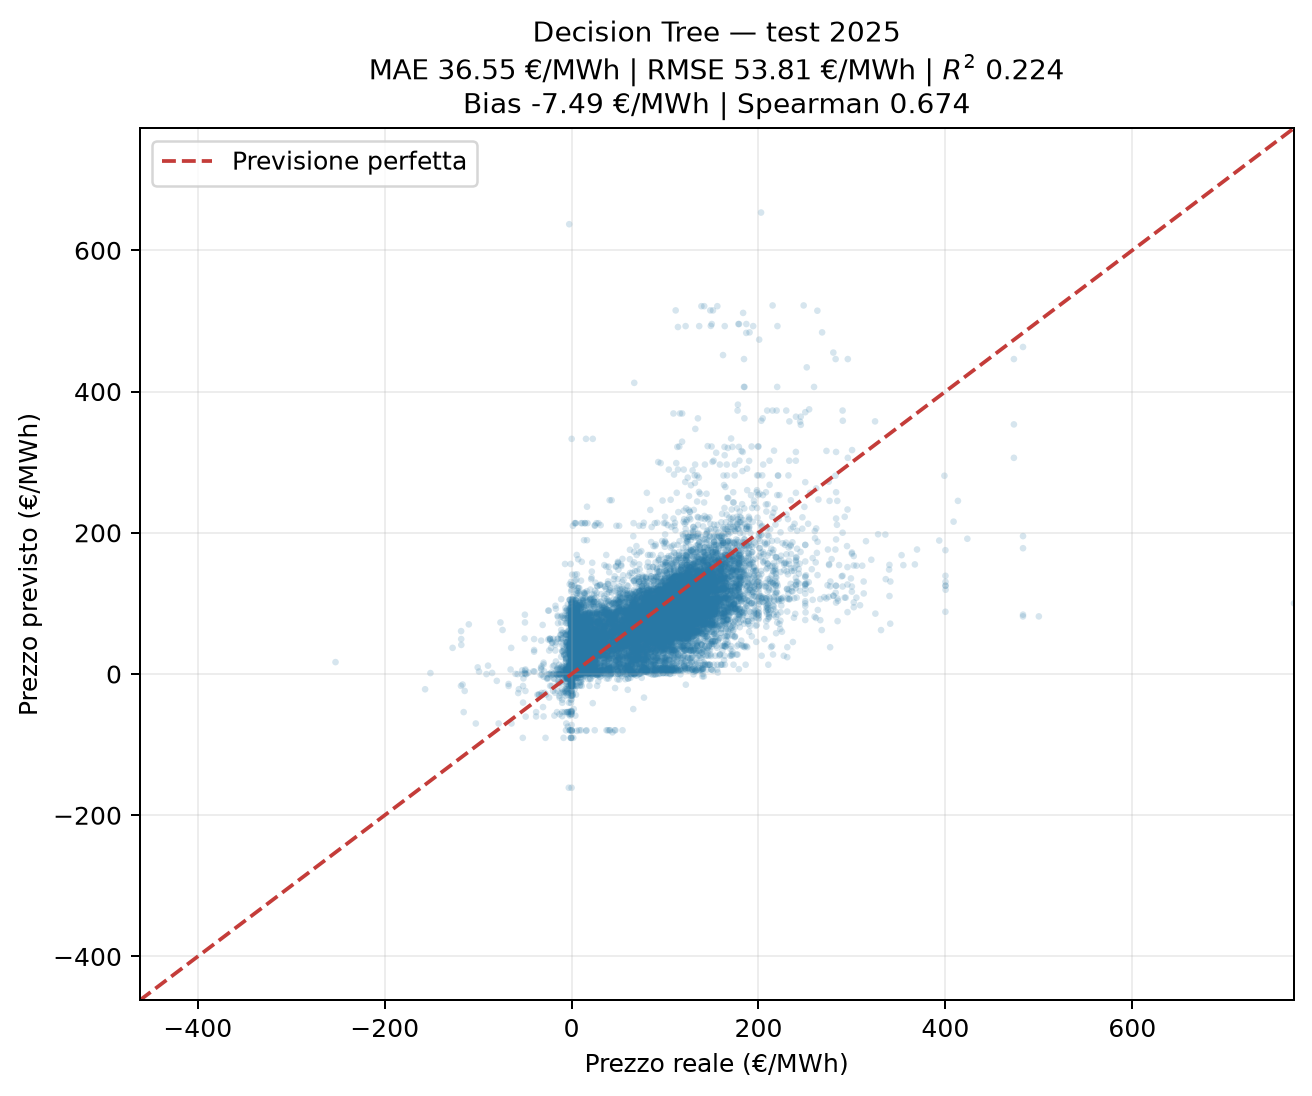
\includegraphics[width=0.78\textwidth]{images/analisi/regressione/decision_tree.png}
    \caption{Prezzi reali e previsti dal Decision Tree sul test gennaio--giugno 2025.}
    \label{fig:reg_dt_test}
\end{figure}

\newpage

\section{K-Nearest Neighbors (KNN)}
Il K-Nearest Neighbors (KNN) è un modello basato sulle istanze: non apprende una funzione globale, ma memorizza il training set e, per ogni nuova osservazione, calcola la distanza dalle osservazioni di training, seleziona le $k$ più vicine e ne aggrega i target. Poiché le variabili hanno scale diverse, la pipeline standardizza le feature prima di calcolare le distanze euclidee; la media dei prezzi dei vicini è pesata in base alla distanza, così i punti più vicini contribuiscono maggiormente. Sono state valutate sul test le configurazioni $k \in \{5,10,30,50,100\}$; per il modello riportato di seguito è stata impostata $k=30$, scelta che nel notebook sperimentale ha offerto il miglior compromesso tra errore e stabilità. La pipeline completa è mostrata nel Codice~\ref{lst:reg_knn}.

\begin{lstlisting}[language=Python, caption={Pipeline KNN, addestramento e previsione.}, label={lst:reg_knn}]
knn = Pipeline([
    ("scaler", StandardScaler()),
    ("knn", KNeighborsRegressor(
        n_neighbors=30, weights="distance", n_jobs=-1
    ))
])
knn.fit(X_train, y_train)
y_pred_knn = knn.predict(X_test)
\end{lstlisting}

\subsection{Metriche sul test}
Il bias negativo segnala una sottostima media. Sul training il modello riproduce quasi perfettamente le osservazioni perché ogni punto trova sé stesso tra i vicini; la generalizzazione è valutata sul test separato.
\begin{table}[htbp]
    \centering\small
    \begin{tabular}{|l|r|r|r|r|r|r|}\hline
    \rowcolor[gray]{0.9} Modello & MAE & MSE & RMSE & $R^2$ & Bias & Spearman \\
    \hline
    KNN ($k=30$) & 30,97 & 1.748,64 & 41,82 & 0,531 & $-8,37$ & 0,777 \\
    \hline\end{tabular}
    \caption{Metriche del KNN con $k=30$ sul test. MAE, RMSE e bias in \euro/MWh; MSE in $(\euro/\mathrm{MWh})^2$.}
    \label{tab:reg_metriche_knn}
\end{table}

\subsection{Grafico delle previsioni}
\begin{figure}[ht!]
    \centering
    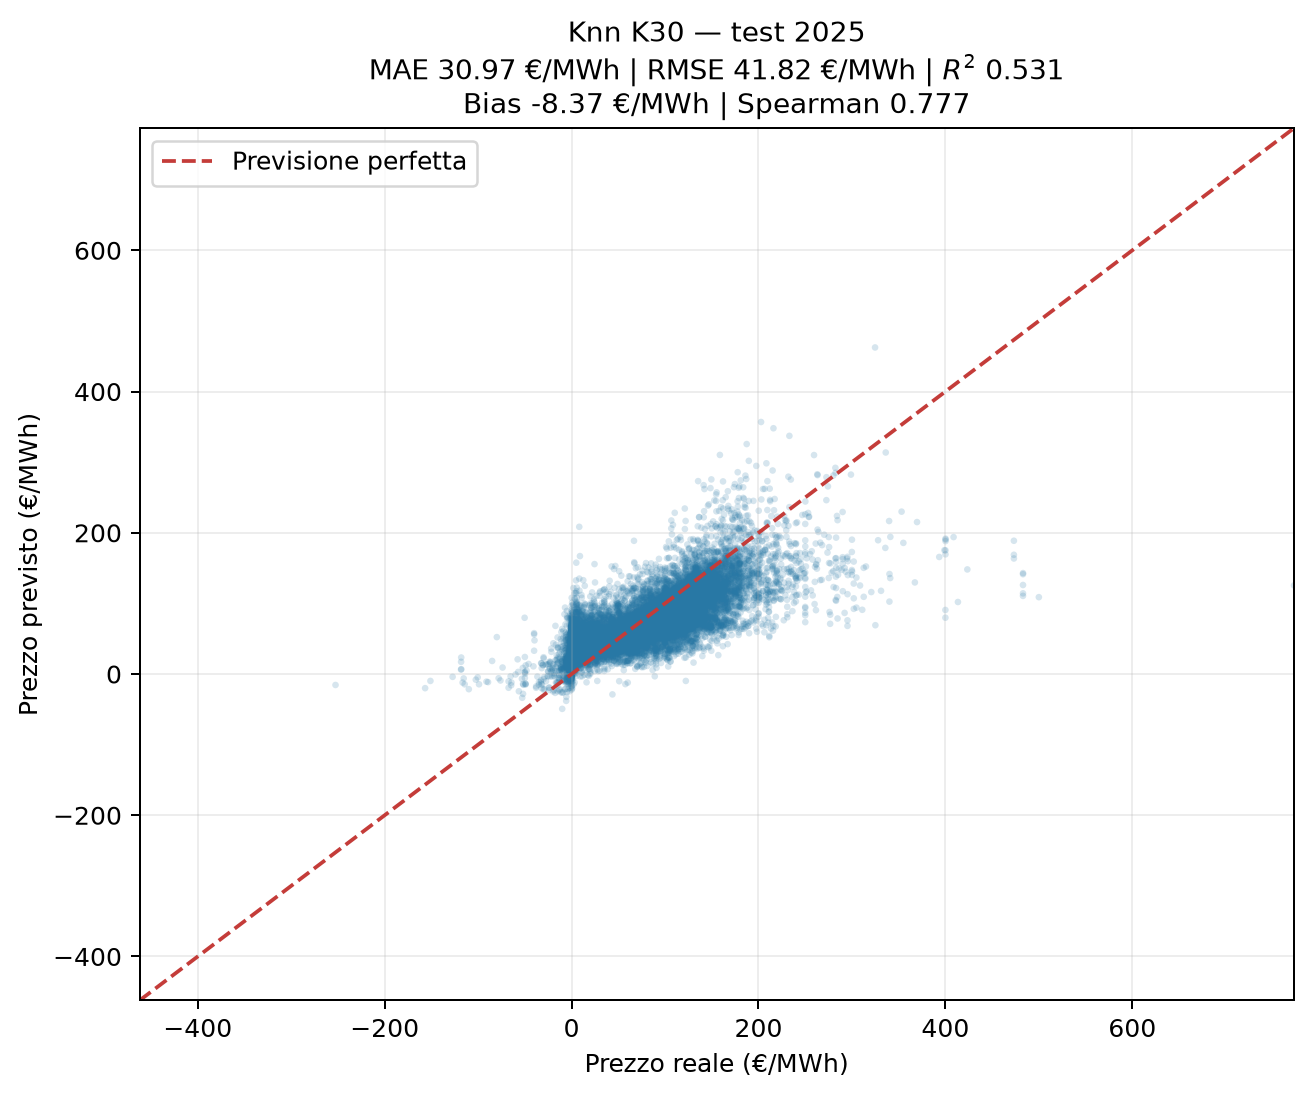
\includegraphics[width=0.7\textwidth]{images/analisi/regressione/knn_k30.png}
    \caption{Prezzi reali e previsti dal KNN con $k=30$ sul test gennaio--giugno 2025.}
    \label{fig:reg_knn_test}
\end{figure}

\newpage

\section{Ridge di grado 1}
La Ridge regression è una variante della regressione lineare che aggiunge una penalizzazione L2 sui coefficienti, con l'obiettivo di ridurre la varianza e prevenire l'overfitting in presenza di molte feature correlate. In questa configurazione di grado 1, le feature numeriche sono standardizzate, mentre le variabili one-hot della zona vengono mantenute senza espansione polinomiale. Il parametro di regolarizzazione è $\alpha=10$. Il codice della pipeline è riportato nel Codice~\ref{lst:reg_ridge1}.

\begin{lstlisting}[language=Python, caption={Pipeline Ridge polinomiale e configurazione di grado 1.}, label={lst:reg_ridge1}]
def make_ridge(degree, alpha):
    num_cols = [c for c in X_train.columns
                if not c.startswith("country_")]
    cat_cols = [c for c in X_train.columns
                if c.startswith("country_")]
    preproc = ColumnTransformer([
        ("poly", Pipeline([
            ("poly", PolynomialFeatures(
                degree=degree, include_bias=False)),
            ("sc", StandardScaler()),
        ]), num_cols),
        ("cat", "passthrough", cat_cols),
    ])
    return Pipeline([
        ("prep", preproc),
        ("ridge", Ridge(alpha=alpha, random_state=42)),
    ])

m = make_ridge(degree=1, alpha=10.0)
m.fit(X_train, y_train)
y_hat = m.predict(X_test)
\end{lstlisting}

\subsection{Metriche sul test}
\begin{table}[htbp]
    \centering\small
    \begin{tabular}{|l|r|r|r|r|r|r|}\hline
    \rowcolor[gray]{0.9} Modello & MAE & MSE & RMSE & $R^2$ & Bias & Spearman \\
    \hline
    Ridge grado 1 & 38,03 & 2.588,08 & 50,87 & 0,306 & $-8,27$ & 0,606 \\
    \hline\end{tabular}
    \caption{Metriche della Ridge di grado 1 sul test. MAE, RMSE e bias in \euro/MWh; MSE in $(\euro/\mathrm{MWh})^2$.}
    \label{tab:reg_metriche_ridge1}
\end{table}

\subsection{Grafico delle previsioni}
\begin{figure}[ht!]
    \centering
    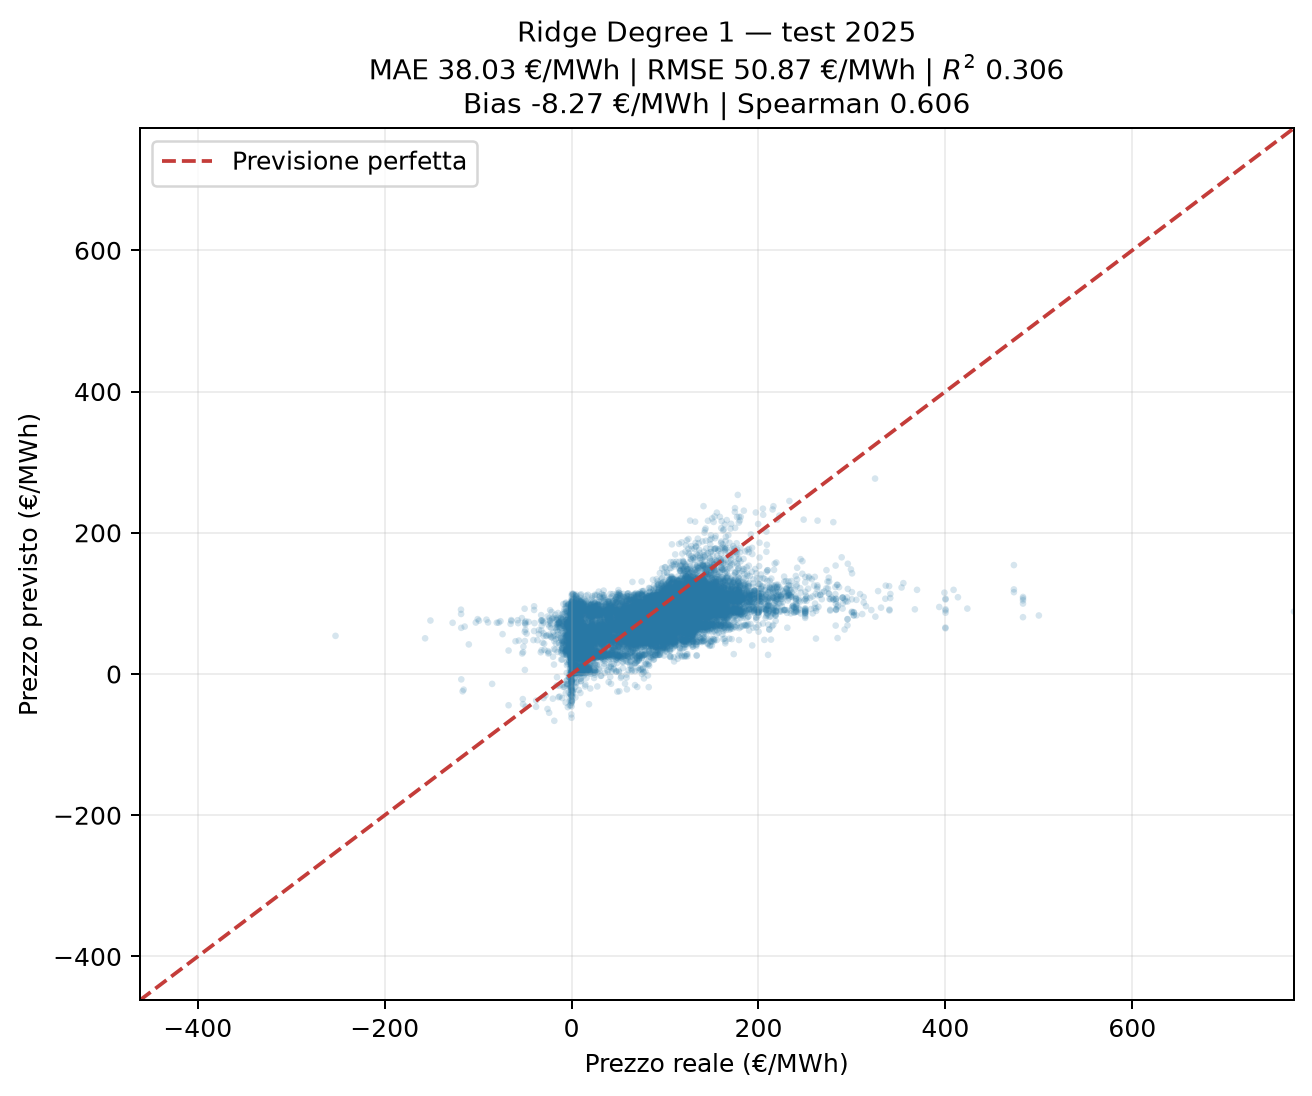
\includegraphics[width=0.51\textwidth]{images/analisi/regressione/ridge_degree_1.png}
    \caption{Prezzi reali e previsti dalla Ridge di grado 1 sul test.}
    \label{fig:reg_ridge1_test}
\end{figure}

\newpage

\section{Ridge di grado 2}
Per la variante di grado 2, le feature numeriche sono espanse includendo termini quadratici e interazioni tra coppie di variabili; le dummy delle zone restano invariate. Questa espansione consente di catturare relazioni non lineari, a costo di un aumento del numero di feature e, quindi, della necessità di una regolarizzazione più forte: $\alpha=100$. Il codice è nel Codice~\ref{lst:reg_ridge2}.

\begin{lstlisting}[language=Python, caption={Configurazione, addestramento e previsione della Ridge di grado 2.}, label={lst:reg_ridge2}]
m = make_ridge(degree=2, alpha=100.0)
m.fit(X_train, y_train)
y_hat = m.predict(X_test)
\end{lstlisting}

\subsection{Metriche sul test}
\begin{table}[htbp]
    \centering\small
    \begin{tabular}{|l|r|r|r|r|r|r|}\hline
    \rowcolor[gray]{0.9} Modello & MAE & MSE & RMSE & $R^2$ & Bias & Spearman \\
    \hline
    Ridge grado 2 & 34,68 & 2.144,89 & 46,31 & 0,425 & $-8,15$ & 0,706 \\
    \hline\end{tabular}
    \caption{Metriche della Ridge di grado 2 sul test. MAE, RMSE e bias in \euro/MWh; MSE in $(\euro/\mathrm{MWh})^2$.}
    \label{tab:reg_metriche_ridge2}
\end{table}

\subsection{Grafico delle previsioni}
\begin{figure}[ht!]
    \centering
    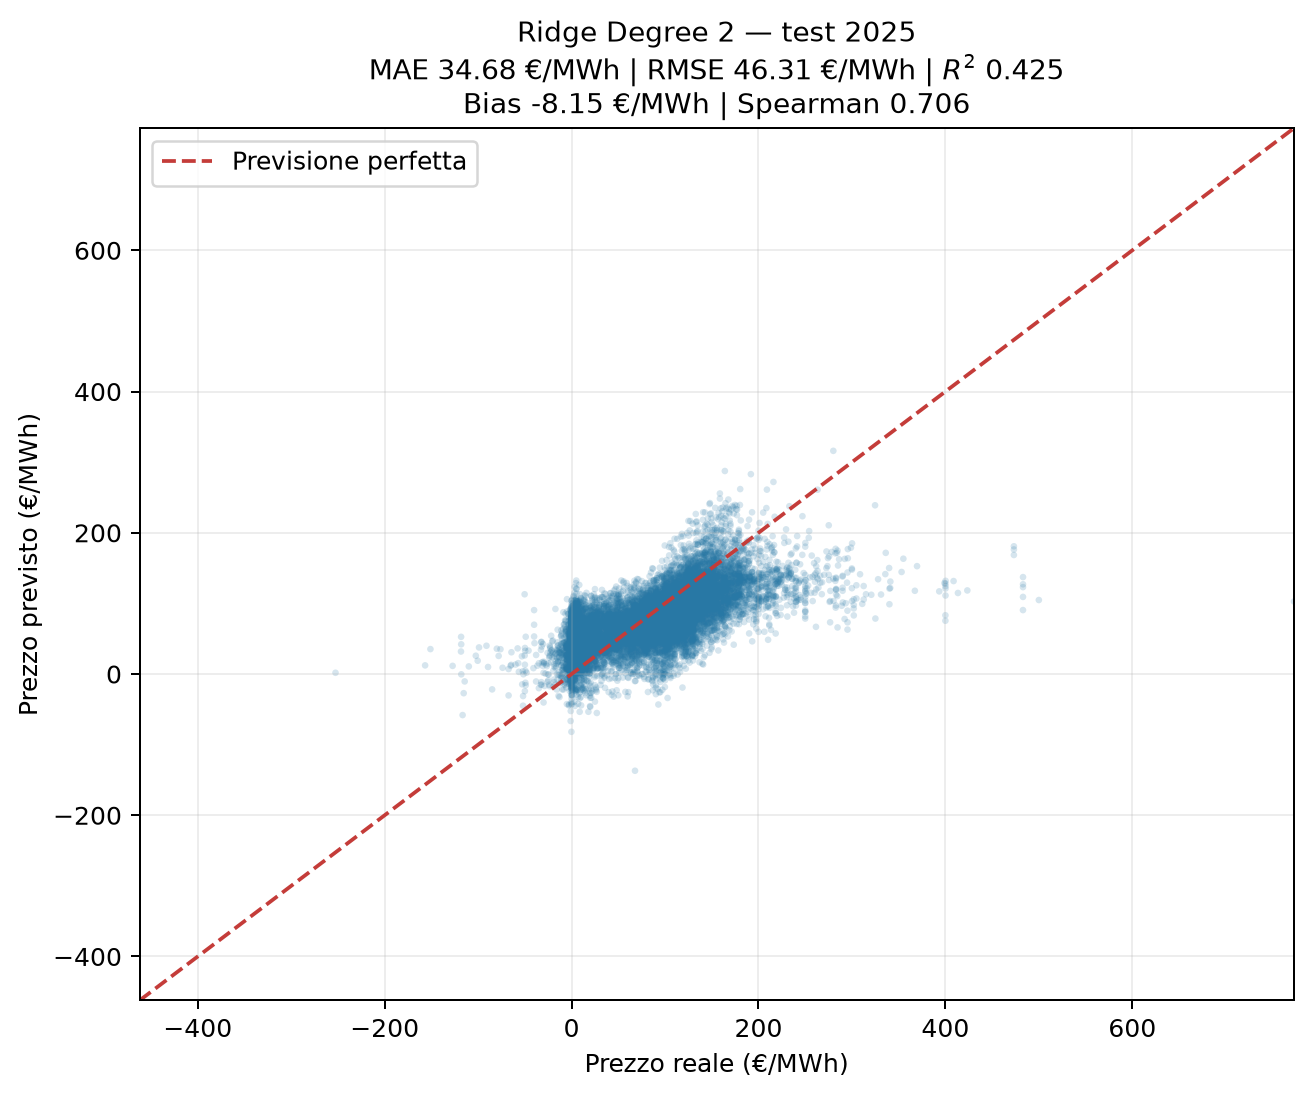
\includegraphics[width=0.7\textwidth]{images/analisi/regressione/ridge_degree_2.png}
    \caption{Prezzi reali e previsti dalla Ridge di grado 2 sul test.}
    \label{fig:reg_ridge2_test}
\end{figure}

\newpage

\section{Ridge di grado 3}
Per la variante di grado 3, l'espansione comprende termini fino al terzo ordine, mantenendo le dummy delle zone senza trasformazione. L'aumento della complessità è compensato da una regolarizzazione più intensa ($\alpha=1000$), necessaria per evitare instabilità numeriche e overfitting. Il codice è nel Codice~\ref{lst:reg_ridge3}.

\begin{lstlisting}[language=Python, caption={Configurazione, addestramento e previsione della Ridge di grado 3.}, label={lst:reg_ridge3}]
m = make_ridge(degree=3, alpha=1000.0)
m.fit(X_train, y_train)
y_hat = m.predict(X_test)
\end{lstlisting}

\subsection{Metriche sul test}
\begin{table}[htbp]
    \centering\small
    \begin{tabular}{|l|r|r|r|r|r|r|}\hline
    \rowcolor[gray]{0.9} Modello & MAE & MSE & RMSE & $R^2$ & Bias & Spearman \\
    \hline
    Ridge grado 3 & 32,71 & 1.930,24 & 43,93 & 0,483 & $-7,34$ & 0,748 \\
    \hline\end{tabular}
    \caption{Metriche della Ridge di grado 3 sul test. MAE, RMSE e bias in \euro/MWh; MSE in $(\euro/\mathrm{MWh})^2$.}
    \label{tab:reg_metriche_ridge3}
\end{table}

\subsection{Grafico delle previsioni}
\begin{figure}[ht!]
    \centering
    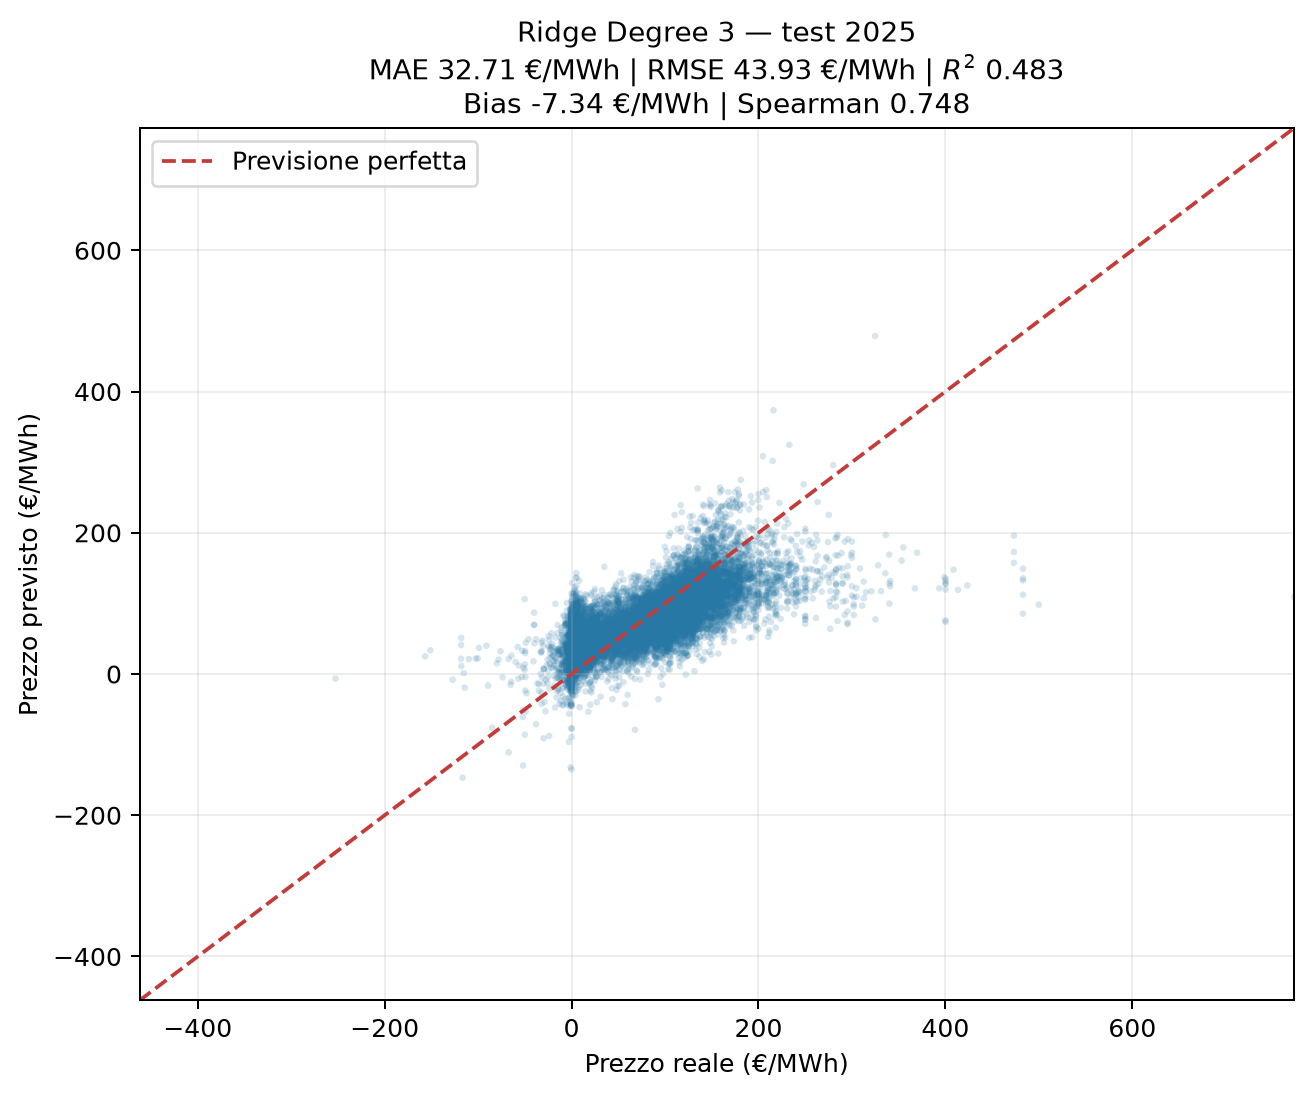
\includegraphics[width=0.7\textwidth]{images/analisi/regressione/ridge_degree_3.png}
    \caption{Prezzi reali e previsti dalla Ridge di grado 3 sul test.}
    \label{fig:reg_ridge3_test}
\end{figure}

\newpage

\section{Confronto dei modelli}
I modelli sono ordinati dal MAE più basso al più alto, usando il MAE come criterio principale: valori inferiori indicano un errore assoluto medio minore. La baseline è inclusa come riferimento e usa la media storica del prezzo per zona, ora e tipo di giorno. La Tabella~\ref{tab:reg_classifica_modelli} riporta anche le altre metriche sul medesimo test.

\begin{table}[htbp]
    \centering\small
    \resizebox{\textwidth}{!}{%
    \begin{tabular}{|r|l|r|r|r|r|r|r|}\hline
    \rowcolor[gray]{0.9} Pos. & Modello & MAE & MSE & RMSE & $R^2$ & Bias & Spearman \\
    \hline
    1 & Random Forest & 29,99 & 1.726,40 & 41,55 & 0,537 & $-7,16$ & 0,775 \\
    2 & KNN ($k=30$) & 30,97 & 1.748,64 & 41,82 & 0,531 & $-8,37$ & 0,777 \\
    3 & Ridge grado 3 & 32,71 & 1.930,24 & 43,93 & 0,483 & $-7,34$ & 0,748 \\
    4 & Ridge grado 2 & 34,68 & 2.144,89 & 46,31 & 0,425 & $-8,15$ & 0,706 \\
    5 & Decision Tree & 36,55 & 2.895,97 & 53,81 & 0,224 & $-7,49$ & 0,674 \\
    6 & Ridge grado 1 & 38,03 & 2.588,08 & 50,87 & 0,306 & $-8,27$ & 0,606 \\
    7 & Baseline & 39,00 & 2.539,44 & 50,39 & 0,319 & $-8,57$ & 0,592 \\
    \hline
    \end{tabular}}
    \caption{Classifica dei modelli per MAE crescente sul test gennaio--giugno 2025. MAE, RMSE e bias in \euro/MWh; MSE in $(\euro/\mathrm{MWh})^2$.}
    \label{tab:reg_classifica_modelli}
\end{table}

Il grafico in Figura~\ref{fig:reg_confronto_modelli} mostra congiuntamente MAE e $R^2$. Il quadrante in alto a sinistra rappresenta la combinazione preferibile: errore assoluto basso e quota di varianza spiegata elevata. La Random Forest offre il compromesso migliore secondo queste due metriche; il KNN è vicino e presenta una correlazione di Spearman lievemente superiore. La baseline ha prestazioni inferiori a tutti i modelli addestrati secondo il MAE.

\begin{figure}[ht!]
    \centering
    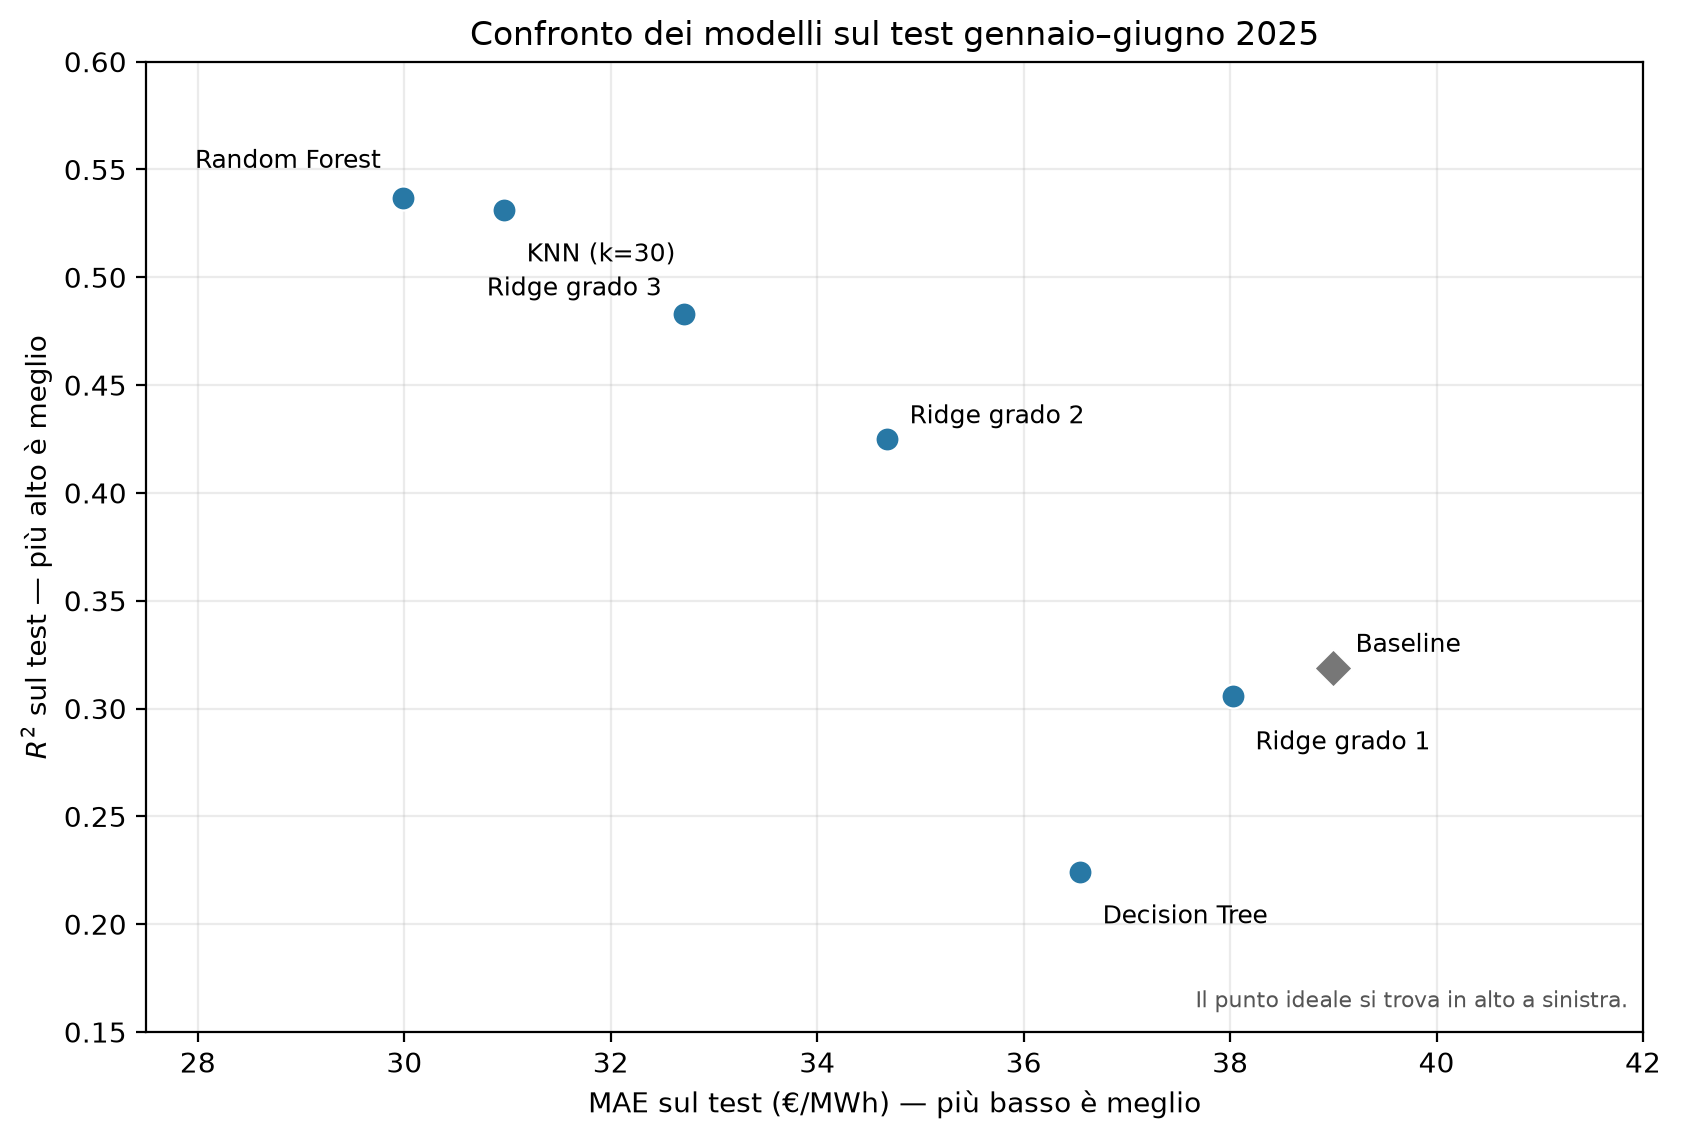
\includegraphics[width=0.82\textwidth]{images/analisi/regressione/confronto_modelli.png}
    \caption{Confronto tra MAE e $R^2$ dei modelli sul test. Un punto più vicino all'angolo superiore sinistro indica prestazioni migliori secondo entrambe le metriche.}
    \label{fig:reg_confronto_modelli}
\end{figure}